\chapter{Attenuation Constant in waveguides}
In this chapter, we will talk about attenuation constant which was studied in the last chapter. In practice, the material with which the waveguide is made, is not an ideal conductor. So, we have ohmic losses in the walls  of the wave guide and also the dielectric which is filling the waveguide may not be an ideal dielectric, and because of that, we may have dielectric losses in the dielectric.

Last time, we saw that the attenuation constant due to two {2} components \textbf{(i) the finite conductivity of the walls and (ii) the finite conductivity of the dielectric filling the waveguide}, which are treated independently. So we calculate the attenuation constants due to each of these components and then we say the total attenuation constant is the sum of the 2 attenuation constants under the assumption that the losses are very small in a good waveguide.

The last time, we calculated attenuation constant due to dielectric material introducing the concept of complex permitivity. So in the dispersion relation, if we replace the dielectric constant by the complex dielectric constant for the medium, then separating the real and imaginary parts, we can get the attenuation constants due to the dielectric losses.

We then develop a frame work for calculating the dielectric constant due to the finite conductivity of the walls and the waveguide.

In this lecture,we will look at two (2) cases of Parallel Plane Waveguide in \textbf{TEM mode} and the other rectangular waveguide \textbf{$\boldsymbol{TE_{10}}$ mode}.

\section{Attenuation Constant For TEM Mode in Parallel Plane Waveguide}

\begin{figure}[h]
\centering
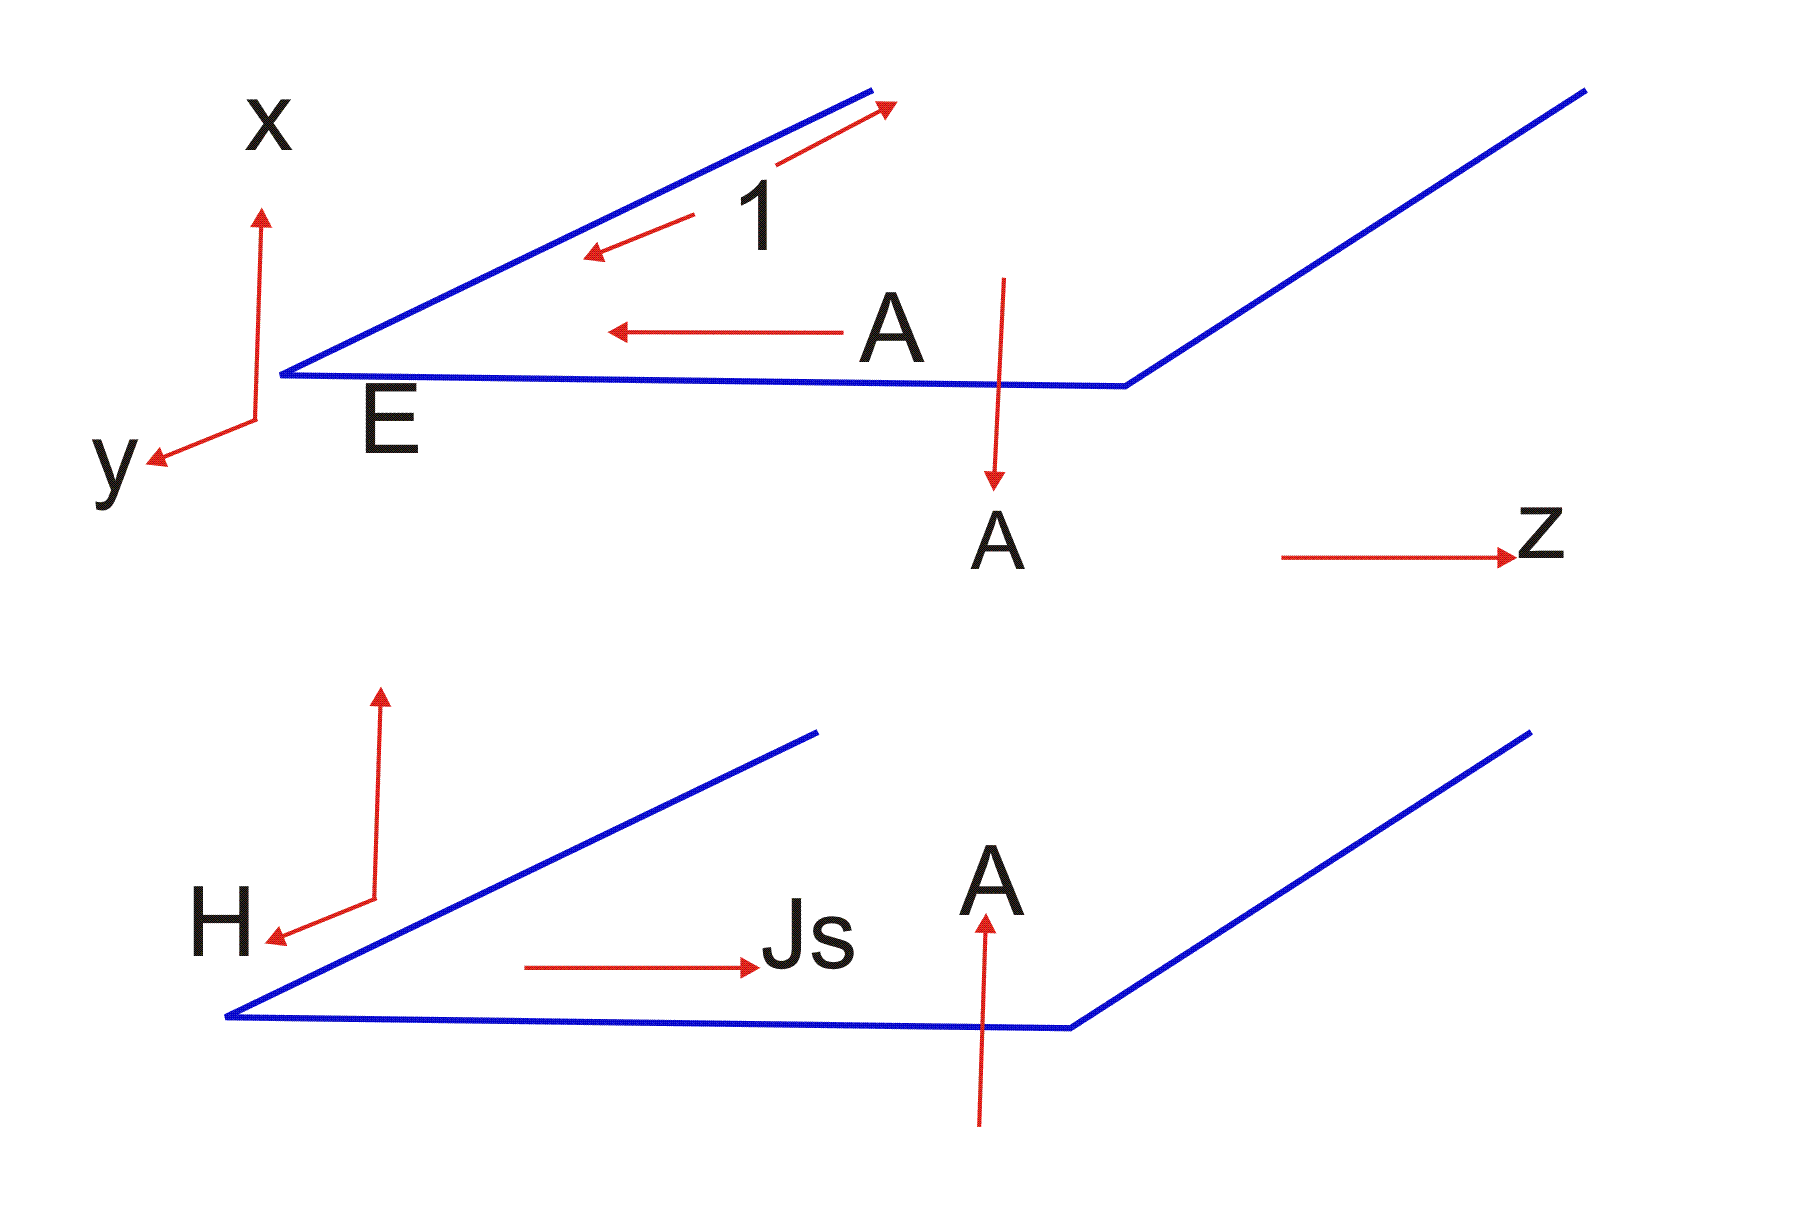
\includegraphics[scale=0.45]{./graphics/lecture2-image-b.png}
\caption{propagation of fields inside a parallel plane waveguide for TEM mode}
\end{figure}

For the calculation of  attenuation constant $\alpha_c$   for TEM in a parallel waveguide to be done, solving for $\alpha_c$  will give us some feel of when we use structures like coaxial cables, parallel wire lines and how the losses are actually calculated. We have seen the calculation of the losses from the knowledge of resistance and conductance in transmission line. However, we ask a question. How do we know the resistance and conductance in this line, s essentially starting from the fields, we can calculate how the losses are going to take place in this conducting surfaces.

Now, let us consider a parallel plane waveguide with wave propagating in the z direction.
%\begin{figure}[h]
%	\centering
%	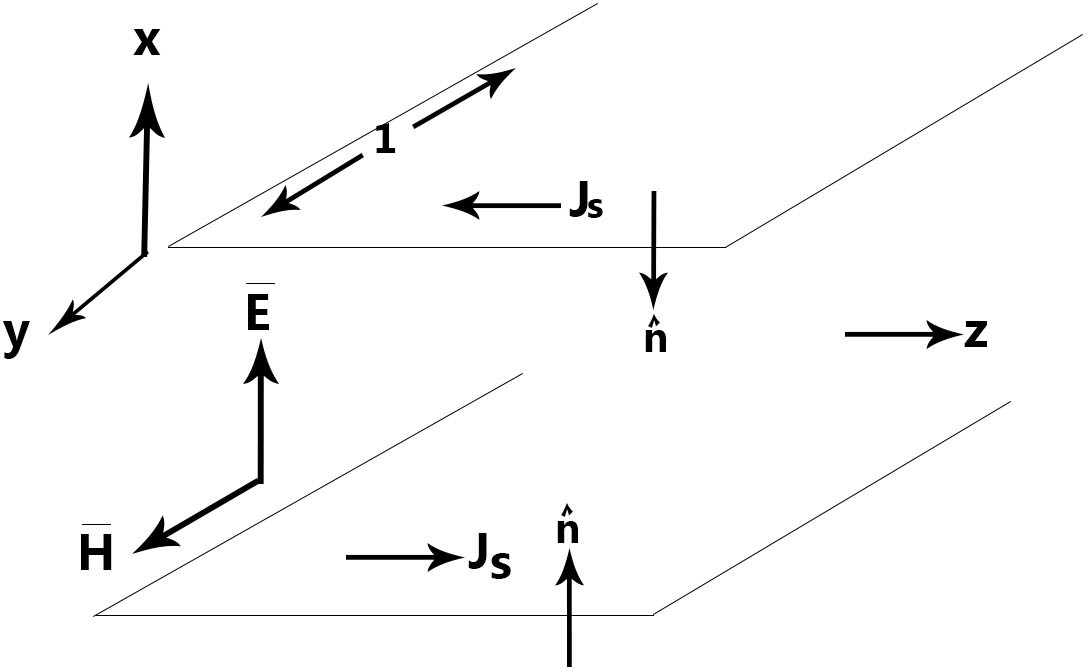
\includegraphics[height=5cm]{411}
%	\vspace{-20pt}
%	\caption{propagation of fields inside a parallel plane waveguide for TEM mode}
%\end{figure}
\begin{figure}[h]
\centering
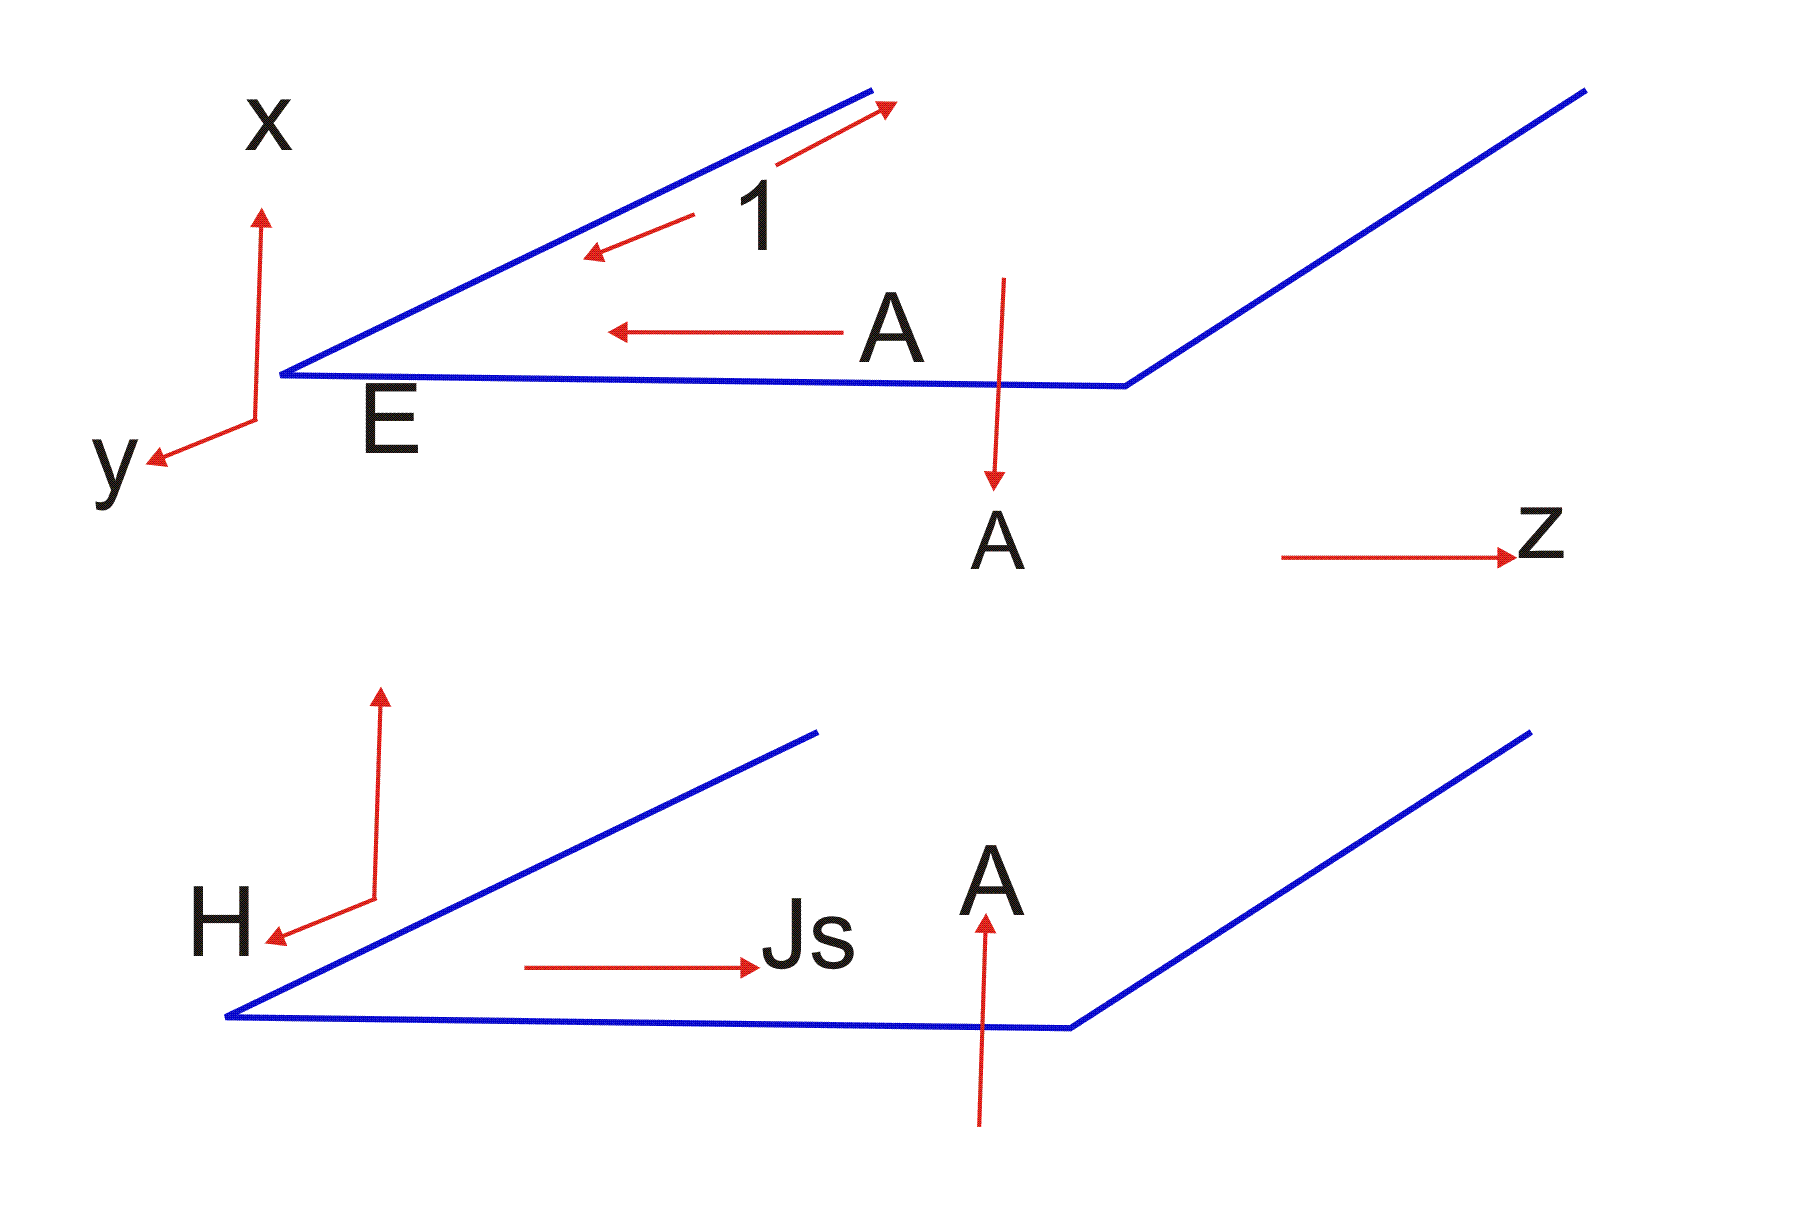
\includegraphics[scale=0.45]{./graphics/lecture2-image-b.png}
\caption{propagation of fields inside a parallel plane waveguide for TEM mode}
\end{figure}
For this case, we say $\overline{E}$ is in the x direction and $\overline{H}$  in the y direction for the coordinate axis. For this mode, the ratio of the $\overline{E}$ and  $\overline{H}$ fields is equal to the intrinsic impedance of the medium filling the waveguide so we have a relation between $\overline{E}$ and  $\overline{H}$

Parallel Plane wave guide $\frac{\overline{E}}{\overline{H}} = \eta $ intrinsic impedance of the medium in the waveguide.

If we express the electric field $\overline{E}$ as some amplitude $E_0$, so that
\begin{equation}
\overline{E} = E_0 e^{-j\beta }\hat{x}
\end{equation}
\begin{equation}
\overline{H} = \frac{E_0}{\eta} e^{-j\beta z}\hat{y}
\end{equation}
Since the waveguide is infinite in the y direction, if we go by the relation
\begin{center}
$\alpha = \frac{\text{power decrease per unit length}}{\text{2 $\times$ total power carried by the waveguide}}$	
\end{center}

to find out the total power carried by the waveguide, then the power will be infinite since the cross section of the waveguide is infinite, y tends to $\infty$. The losses will be infinite and we will not get a definite or meaningful answer.

So we define the $\alpha_{c}$ by the unit width of this waveguide. We take a piece of the waveguide which is of unit length in the y direction i.e (1) in the y direction. What is the powerloss in the unit length of the waveguide? What is the power carried by unit width of the waveguide? From there we can calculate the attenuation constant $\alpha_{c}$ of the waveguide. 

Now we have $\overline{H}$ which is not varying as a function of y, it is constant for y, with amplitude $\frac{E_0}{\eta}$. On top and bottom walls, the magnetic field will be in the y direction.\\\\ As we saw last time, the normal to the surface bounding the electromagnetic wave is as shown. Going by $\hat{n}\times\overline{H}=\overline{J_s}$, we have the direction of $\overline{J_s}$ shown by the arrows. The amplitude of $\overline{J_s}$ is exactly the same amplitude with $\frac{E_0}{\eta}(\overline{H})$. Now that we have visualized the fields and currents inside the waveguide, then, those fields are going to move with the phase velocity inside the waveguide in the z direction.

So, all the  quantities, $\overline{E}, \overline{H}$ are going to have a sinusoidal variation as a function of time. If we consider any location on the conducting plane, the fields, $\overline{E}, \overline{H}$ and the current $\overline{J_s}$ are going to vary sinusoidally as a function of time. So, if we take the peak amplitude, $E_0$ and $\frac{E_0}{\eta}$ of ($\overline{E}$ and $\overline{H}$ ) and find out the RMS value of the fields and the RMS value of the surface currents,we can get the average power lost and average power carried by the waveguide. So for unit width of the waveguide,the power carried by the waveguide per unit width is $\frac{Re}{2}(E \times H^*)$ integrated over the cross section of height (a or d) and width of the waveguide = 1. So, let us say the height of the waveguide is given as a, then the power carried by the waveguide per unit width.

\begin{equation}
W=\int_{x=0}^{a}\int_{y=0}^{1} \frac{1}{2}Re{(\overline{E} \times \overline{H})dxdy}	
\end{equation}
$\overline{E}$ is in x direction, $\overline{H}$ is in y direction, so the power flow is in the z direction. $\overline{E} \times \overline{H}^*$ is we take this to be $\overline{E} \times \frac{\overline{E}}{\eta}$. If we consider the dielectric filling the waveguide is an ideal dielectric, $\eta$ is a real quantity. \\
So, essentially,

\begin{center}
$W$ = $\int_{x=0}^{a}\int_{y=0}^{1}\frac{1}{2}Re(E_0 \frac{E_0^*}{\eta})dxdy$

\end{center}
\begin{equation}
= \frac{\left|E_{0}\right|^2}{2\eta}\int_{x=0}^{a}\int_{y=0}^{1}dxdy = \frac{|E_0|^2a}{2\eta}
\end{equation}


This is the total power carried by the TEM mode per unit width of the waveguide. The second quantity we need is the power loss per unit length of the waveguide. As we have seen earlier, when we go to the concept of what we call surface resistance, if we know the conductivity of the boundary, we can calculate the surface resistance. From the surface resistance, we can calculate the power loss per unit area.
\begin{equation}
=\frac{1}{2}R_s|\overline{J_s}|^2 
\end{equation}

So power loss per unit length 
$ =-(\frac{dw}{dz}) $

This is integrated over the area made by length in z direction and breadth im y direction of 1  unit. We make use of length 1 in z i.e unit length. So area is from 0 to 1 in z and 0 to 1 in y. $ \overline{J_s} $ is the same as a magnetic field, its magnitude will be $ \frac{E_0}{\eta} $ and H* will have a sinusoidal variation in time, so per unit length. If we calculate this value and integrate over the unit area 
, that would give the total loss per unit area of the wall. Since there are 2 walls, the total loss will be doubled. For each wall we calculate
power loss per unit length; 
\begin{equation}
-\frac{dw}{dz}= 2 \int_{y=o}^{1} \int_{z=0}^{1}\frac{1}{2}R_s|\overline{J_s}|^2dydz
\end{equation}
Note: The 2 indicates the 2 walls of the waveguide. 

If we recall, the $R_s$ was the real part of the intrinsic impedance of the conducting wall. For the conducting wall,
$$\eta_c = \sqrt{\frac{j\omega\mu}{\sigma}}= \sqrt{\frac{\omega\mu}{2\sigma}}+j\sqrt{\frac{\omega\mu}{2\sigma}}$$

Recall:
\begin{center}
$\sqrt{\frac{\omega\mu}{2\sigma}}=R_s$	
\end{center}
which is the surface resistance. Also,
\begin{center}
$j\sqrt{\frac{\omega\mu}{2\sigma}}=X_s$
\end{center}
which is the Surface Reactance.
\begin{equation}
\eta_c = R_s + X_s.
\end{equation}
We are interested in power loss here, so that we can substitute for $R_s$ in $\frac{dw}{dz}$ equation to have
\begin{center}
$-(\frac{dw}{dz})=\sqrt{\frac{\omega\mu}{2\sigma}}\times\frac{|E_0|^2}{\eta}$
\end{center}
\begin{equation}
W=\frac{|E_0|^2 a}{2\eta}
\end{equation}
This equation is the power loss per unit length of the waveguide. So, we have the quantities which are needed for the  calculation of attenuation constant .
Attenuation constant 
\begin{center}
$$\alpha_c = \frac{\sqrt\frac{\omega\mu}{2 \sigma}\times\frac{|E_0|^2}{\eta}}{2 \times \frac{|E_0|^2 a}{2 \eta}}$$

$$= \frac{2}{a}\sqrt{\frac{\omega\mu}{2\sigma}}=\frac{1}{a}\sqrt{\frac{\omega\mu}{2\sigma}}$$	
\end{center}
Thus, we get the attenuation constant of the parallel plane wave guide as

\begin{equation}
\alpha_c=\frac{1}{a}\sqrt{\frac{\omega\mu}{2\sigma}}
\end{equation}
$\omega$ is the frequency, $a$ is the height of the waveguide, $\mu$ is the permeability of the dielectric, and $\sigma$ is the conductivity of the parallel planes.Somethings can be observed from this equation, 
\begin{enumerate}[(i)]
\item The attenuation constant is inversely proportional to the height of the waveguide. This makes sense, because if we consider the parallel plane waveguide, since magnetic field does not vary as a function of height, no matter the separation of the two planes, the power loss per unit length is the same as it does not change. However, the power carried by the waveguide is affected in that it increases. But the power loss per unit length does not change and it is small. As a result, the attenuation constant reduces with increasing height, a.
\item The attenuation constant is inversely proportional to the conductivity, $\sigma$. That, we understand, because if you have a good conductor, as the conductivity becomes large, the attenuation gets smaller since there will be less loss in the limit, $\sigma$ tends to $\infty$, $\alpha_{c}$ tends to 0. So, a waveguide made of ideal conductor will have 0 attenuation constant. The important thing to note is that attenuation constant $\alpha_{c}$ is a function of frequency $\omega$. As $\omega$ increase, the attenuation constant $\alpha_{c}$ increases.
\item Attenuation constant is directly proportional to frequency, in that, as frequency increases, attenuation constant increases and vice versa. At high frequencies, the loss becomes excessive and signal cannot be fed effectively. In coaxial cables, at low frequencies, the attenuation constant is manageable whereas high frequencies create a low-pass filtering effect smoothening signals because of too much losses. When the same structure is used to carry signal at high frequencies, the loss becomes excessive, so signal cannot be transmitted efficiently from one point to the other. Looking at another angle, suppose we had to send a broadband signal using this structure, i.e. the signal occupies very large bandwidth, the lower end of the frequency spectrum will go efficiently, but the higher end of the spectrum will not go efficient;y. Its amplitude will be reduced.
\end{enumerate}
At low frequencies  the attenuation  constant  is manageable but when we use the same structures to carry signals at high frequency, the  loss becomes excessive and the signal cannot be transmitted  efficiently from one point to the other. We can also see this from another angle, that suppose we need to send a broadband signal using this  structure i.e if the signal occupy very large bandwidth, the lower  end of the frequency  spectrum will go efficiently but the higher end of the frequency spectrum  will not go efficiently.Its amplitude  would be reduced and the wave guiding structure has an effect like that of a LOW PASS FILTER. So the signal is distorted  as if it was pass through a low pass filter. 
Whenever  there is a guiding structure, invariably there is low pass filtering  and a distorted signal I.e there will be blurring  of the sharp edges of the signal in time. Signals get smoothed out because of low pass filtering action caused by lossy behaviour of the waveguide. Conductor loss varies with frequency and so an increase  in frequency will lead to high loss for the same wave guide structure. 

\section{Transverse Electric Mode (TE10)}
Since this is the mode that will propagate inside a rectangular waveguide. Recall for
$TE_{10}$ mode
\begin{center}
$\frac{E_x}{E_z}=0$

$H_y=0$	
\end{center}
$$
E_{x} = E_{z} = H_{y} = 0
$$	
$$
E_{y} = \dfrac{-j\omega\mu a }{\pi} C\sin \dfrac{\pi a}{x} e ^{-j\beta z}
$$
$$
H_{x} = \dfrac{-j\omega a}{\pi} C \sin\dfrac{\pi a}{x}
e^{-j\beta z} 
$$

$$
H_{z} = C\cos \dfrac{\pi x}{a} e^{-j\beta z}
$$


Last time we saw the current distribution because of these fields. Now we use  these fields to calculate power carried by the waveguide, the loss in the four walls of the wave guide and then we calculate the attenuation constant.\\\\ 
From the waveguide shown below

\begin{figure}[H]
\centering
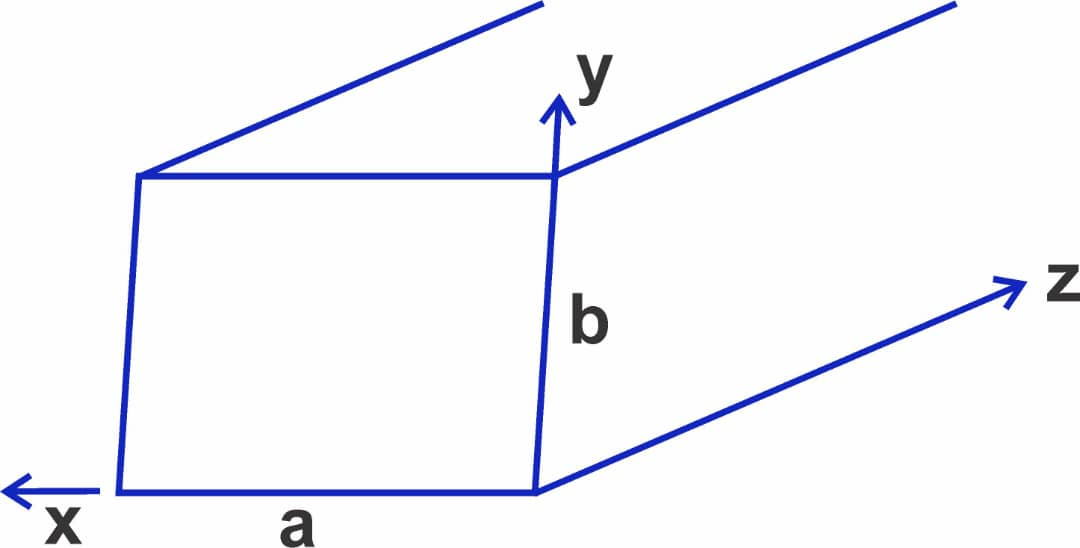
\includegraphics[width=1\linewidth]{./graphics/lecture-image-21.jpg}
\caption{propagation inside a rectangular waveguide2}
\end{figure}


First we calculate the total power since the area of the cross section is known. We take per unit length of the waveguide in the z direction. Calculate the loss per unit length, from same argument, at every location the field is going to sinusoidally as a function of time.
We take the peak value of the magnetic field and just take  the r.m.s value from there and then  we can calculate for the power loss by integrating over the length of the waveguide.
First we take total power or power carried:
\begin{center}
$W= \int_{x=0}^{a}\int_{y=0}^{b}\frac{1}{2}R_e(\overline{E} \times H^*)dxdy$
\end{center}
$E_y$ has -j and $H_x$ has j, $E_y\times H_x^*=$ give -j$\times(-j)=-1$\\
$E_y\times H_2^*$ gives imaginary value. So only $E_y\times H_x^*$ gives real power flow. 

 So,
\begin{center}
$W= \int_{x=0}^{a}\int_{y=0}^{b}\frac{1}{2}R_e(E_yH_x^*(-\hat{z}))+(E_yH_z^*)dxdy$
\end{center}
\begin{center}
$W= \int_{x=0}^{a}\int_{y=0}^{b}\frac{1}{2}\frac{\omega\mu a}{\pi}.\frac{\beta a}{\pi}c^2sin^2(\frac{\pi x}{a})dxdy$
\end{center}
\begin{center}
$=\frac{\omega\mu\beta a^2c^2}{2\pi^2}.b\int_{x=0}^{a}sin^2(\frac{\pi x}{a})dx$
\end{center}
\begin{equation}
=\frac{\omega\mu\beta a^3bc^2}{4\pi^2}
\end{equation}
By knowing the fields for TE10 mode,we can calculate the total  power  carried by the wave guide. Power calculation for the loss in the waveguide is rather tedious  because in the case of parallel plane waveguide,we had only two planes and the current distribution was simple and the current  was moving only in the z direction, so we could integrate very easily. 
For the case of the rectangular waveguide, the current which is flowing on the surface is rather complicated.
We showed last time that it was some kind of blooming and closing flower on the two alternate planes of the rectangular waveguide. 

%\begin{figure}[h]
%	\centering
%	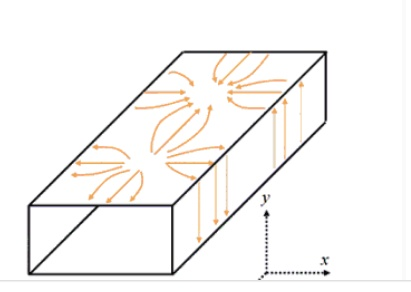
\includegraphics[scale=0.5]{ppw2}
%	\caption{the direction of magnetic and electric fields viewed from the surface of a rectangular waveguide}
%\end{figure}
\begin{figure}[H]
\centering
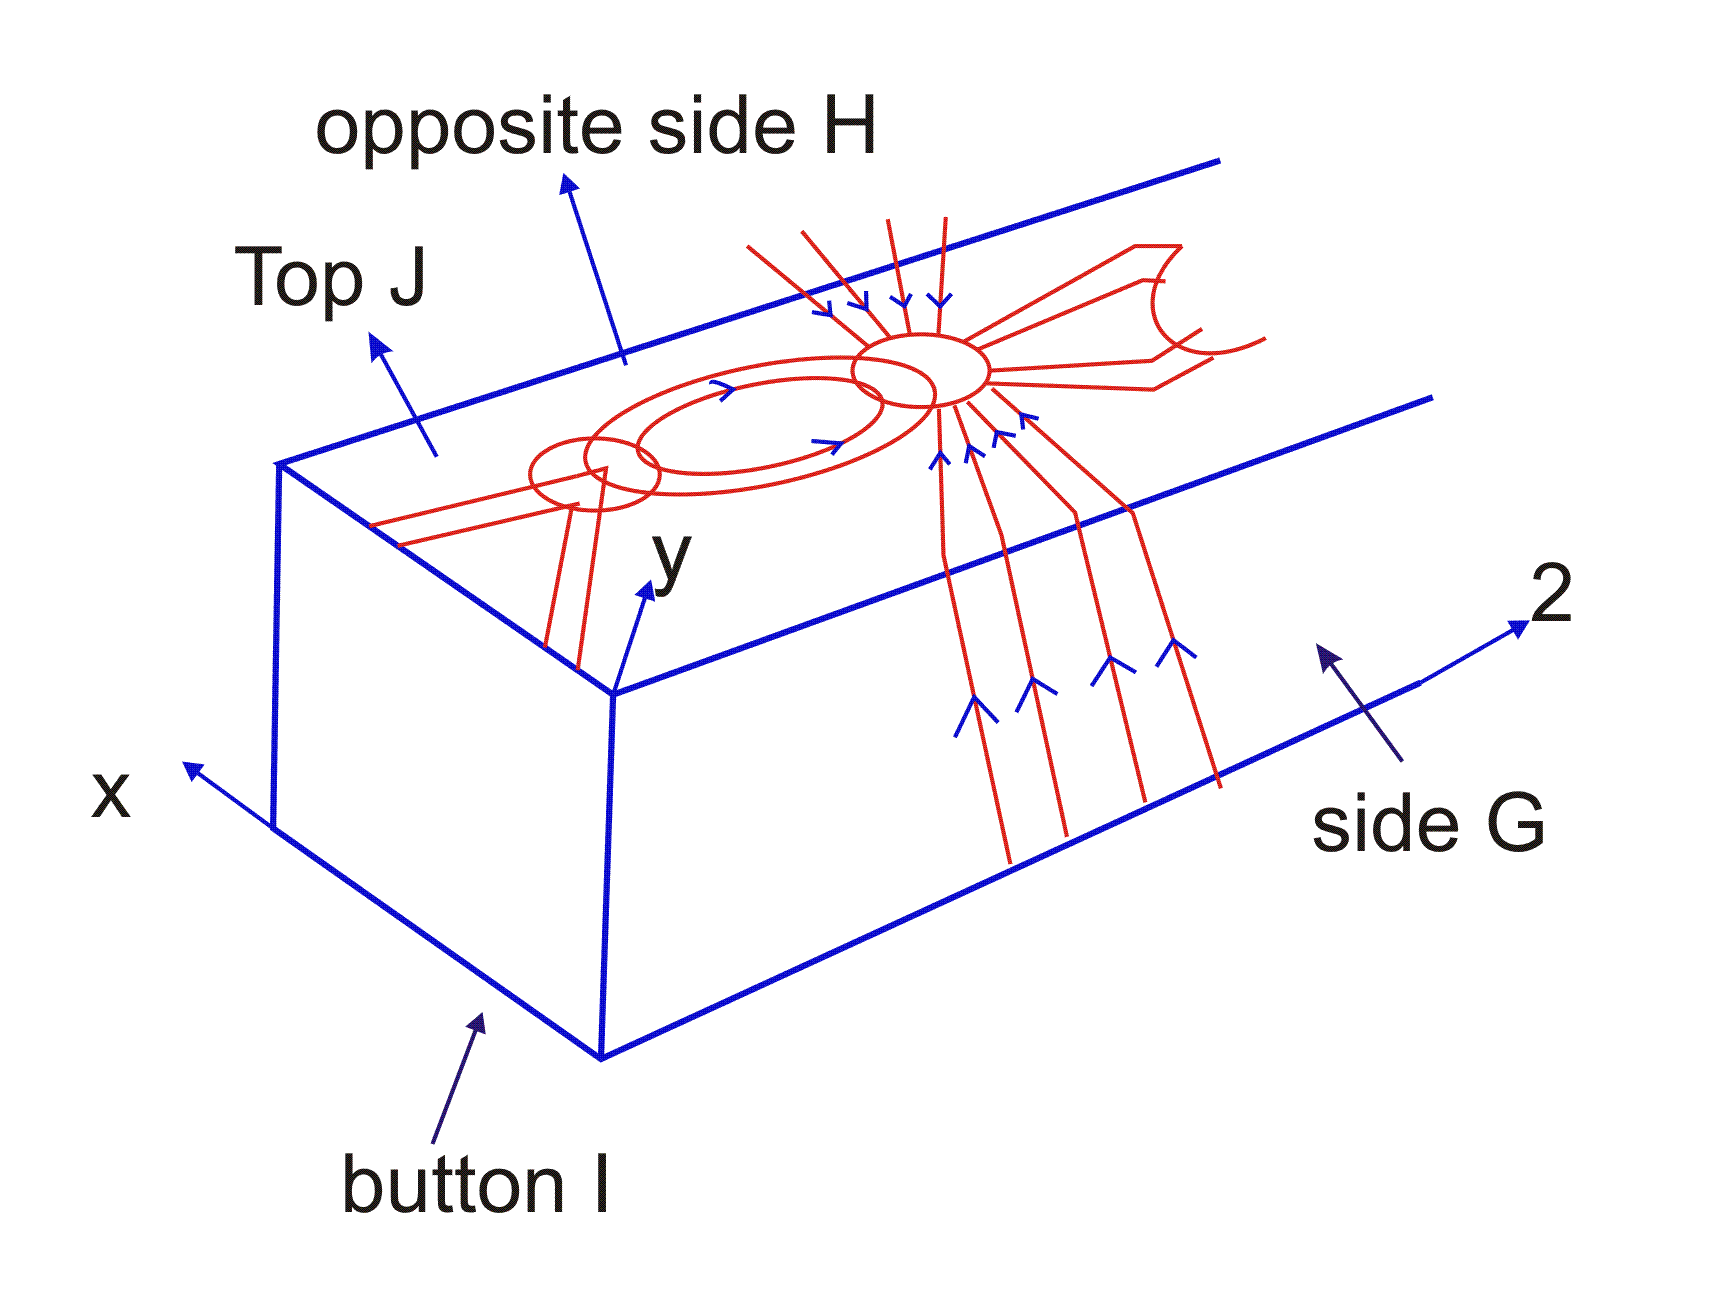
\includegraphics[width=1\linewidth]{./graphics/lecture2-image-a.png}
\caption{the direction of magnetic and electric fields viewed from the surface of a rectangular waveguide}
\end{figure}

On side G, the component of magnetic field was frequency and it varies as a function  of y. So on side G,we have a current that varies only with y. On the top and bottom  surface, we have$H_x$ $H_2$ present. 
$H_x$ is non zero at y=0 and y=b.
Hence on the top, we have current direction in x and z.
On side G and H,we have current that are only y oriented. So,
$$\overline{J_s}|_{x=0} = \overline{J_s}|_{x=a} = H_z|_{x=0 \ or \ x=a}=C$$
from here we can calculate the loss of the waveguide, but we have now the two component of the current.\\ One that is  Z oriented on top and bottom wall and the other x oriented  on top and bottom  wall. So If we are to find the total current  on these walls, we have to have a vector sum of the two currents on the top and bottom surface of the walls of the waveguide. From there we can calculate the total loss  of the waveguide.
First let us calculate the loss for the sidewalls G and H. 
For the side wall $H_2=(cos(\frac{\pi x}{a})e^{j\beta z}$ at x=a gives current inside it which does not vary with y and at x=0 will help give current in G ($\hat{n} \times \overline{H}$) which does not vary with y. Also, $e^{j\beta z}$ gives sinusoidal variation but we are interested in the amplitude,hence instead of writing $ce^{-j\beta z}$ (with x=0 or x=a) we take just C term. So, the current  on the vertical  walls are
\begin{center}
$J_s|_{x=0} = J_s|_{x=a} = H_z|_{x=0 or x=a} = C$	
\end{center}
x=0 represent  wall G and X=a represent wall H. The magnetic field on this side wall
\begin{center}
$H_2=cos(\frac{\pi x}{a}) e^{-j\beta z}$	
\end{center}
does not vary with y. So if we calculate the loss in the two walls per unit length of the waveguide, It is
\begin{equation}
W_L|_{\text{verticalwalls}} = 2\int_{y=0}^{b}\int_{z=0}^{1}\frac{1}{2}R_s|\overline{J_s}|^2dydz
\end{equation}
Recall $\overline{J_s}$ is given by c which we can substitute  in hence to have
\begin{equation}
=R_s|c|^2b
\end{equation}
So calculation  of the loss in the vertical walls is quite simple because we have one component of the surface current which is y oriented. 
However, when we go to the top surface, we have two magnetic field components on the top and bottom surface $H_x$ and $H_z$. So we have to find the total current on this surface and then calculate for the loss for the top and bottom  surfaces. 

\section{HORIZONTAL WALLS} 
$\overline{J_s}$ is a vector  quantity  now as there are two  components in x and z
\begin{center}
$|\overline{J_s}|_{y=0(bottom)} = |\overline{J_s}|_{y=b(top)} = |H|_{y=0}$
$=(|\overline{H}_x|^2 + (|\overline{H}^2 )$
\end{center}
$|\overline{H}|$ is the magnitude  of the total component made up of Hx and Hz.\\\\

Recall
\begin{center}
$\overline{H_x} = \frac{j\beta a}{\pi}Csin(\frac{\pi x}{a})e^{j\beta z}$
\end{center}
\begin{center}
$H_z=Ccos(\frac{\pi x}{a})e^{j\beta z}$
\end{center}
They are not varying as a function of y, so they are the same at y=0 or at y=b i.e at top and bottom  plane which are the two horizontal walls.
\begin{center}
$W_L|_{HOR} = 2\int_{x=0}^{a}\int_{z=0}^{1}\frac{1}{2}R_s(|H_x|^2 + |H_z|^2)dxdz$
\end{center}
\begin{center}
$=\int_{x=0}^{a}\int_{z=0}^{1}R_s ((\frac{\beta a}{\pi})^2C^2 \times sin^2(\frac{\pi x}{a})+ C^2cos^2(\frac{\pi x}{a}))dxdz$	
\end{center}
Solving  this integral we get
\begin{equation}
W_L|_{HOR} = \frac{R_S|c|^2 a}{a}\left(\left(\frac{\beta a}{\pi}\right)^2 +1\right)
\end{equation}
$W_L|_{HOR} + W_L|_{VER}$ =total loss,=losses in horizontal Walls + losses In vertical walls
\begin{center}
$W_L=-\frac{dw}{dz}=W_L|_{VER}+W_L|_{HOR}$	
\end{center}
\begin{center}
$=R_s|C|^2b+\frac{R_s|C|^2a}{2}[(\frac{\beta a}{\pi})^2+1]$	
\end{center}
We can write this in terms of frequency and the cut off frequency of the mode, because we know cut off frequency  is related to the dimension of the waveguide=
\begin{center}
$=R_s|C|^2 (b + \frac{a}{2} + \frac{a}{2}(\frac{\beta a}{\pi})^2)$	
\end{center}
\begin{center}
$ =R_s|C|^2(b+\frac{a}{2}(1+(\frac{\beta a}{\pi})^2)$	
\end{center}
Recall equation for rectangular waveguide:  
\begin{center}
$\beta=\sqrt{{\omega}^2\mu\epsilon-(\frac{m\pi}{a})^2-(\frac{n\pi}{b})^2}$	
\end{center}
\begin{equation}
\beta = \sqrt{\omega^{2} \mu\epsilon-\omega_c^{2} \mu\epsilon}
\end{equation}
with
\begin{center}
$\omega_c^2\mu\epsilon=(\frac{m\pi}{a})^2+(\frac{n\pi}{b})^2$	
\end{center}
For $TE_{10}$, m=1, n=0
\begin{center}
$\omega_c^2\mu\epsilon=(\frac{\pi}{a})^2$,	
\end{center}
\begin{center}
$\beta^2=\omega^2\epsilon-\omega_c^2\epsilon$  or  $\beta^2 + \omega_c^2\mu\epsilon$	
\end{center}
\begin{center}
$= \omega^2\mu\epsilon$	
\end{center}
\begin{center}
$\frac{\beta^2}{\omega_c^2\mu\epsilon}+1=\frac{\omega^2\mu\epsilon}{\omega_c^2\mu\epsilon}=(\frac{f}{f_c})^2$	
\end{center}
\begin{equation}
= 1+ \frac{\beta^2}{\omega_c^2\mu\epsilon}	
\end{equation}
but $\omega_c^2\mu\epsilon=(\frac{\pi^2}{a})$  with  m=1, n=0. From 
\begin{center}
$\omega_c^2\mu\epsilon=(\frac{m\pi}{a})^2 + (\frac{n\pi}{b})^2$	
\end{center}
\begin{center}
$(\frac{f}{f_c})^2= 1+\frac{\beta^2}{(\frac{\pi}{a})^2}$	
\end{center}
\begin{equation}
=1+ (\frac{\beta a}{\pi})^2	
\end{equation}
\begin{center}
$R_s|C|^2 (b+\frac{a}{2}(1+(\frac{\beta a}{\pi})^2)$	
\end{center}
\begin{center}
$=R_s|C|^2(b+\frac{a}{2}(\frac{f}{f_c)}^2)$	
\end{center}
Hence the total loss in the four walls in terms of cut off frequency is
\begin{equation}
W_L=R_s|C|^2[b+\frac{a}{2}(\frac{f}{f_c})^2]	
\end{equation}
So,we know the two things which are needed are: the total power carried by the waveguide which we got and the power loss per unit length of the wave guide. As we saw once we know these two quantities, then we can get attenuation  constant for the waveguide and that will be:
and 
\begin{equation}
W_L=-(\frac{dw}{dz})= R_s|C|^2[b+\frac{a}{2}(\frac{f}{f_c})^2]	
\end{equation}
and
\begin{equation}
W=\frac{\omega\mu\beta a^3bc^2}{4\pi^2}
\end{equation}
\begin{equation}
\alpha_{c}=\frac{-\frac{dw}{dz}}{z\times w}=\frac{R_s|C|^2(b+\frac{a}{2}(\frac{f}{f_c})^2)}{2\times\frac{\omega\mu a^3bc^2}{4\pi^2}}
\end{equation}
Recall:
\begin{center}
$\beta=\sqrt{\omega^2\mu\epsilon-\omega_c^2\mu\epsilon}$	
\end{center}
\begin{center}
$\beta=\omega\sqrt{\mu\epsilon}\sqrt{1-(\frac{f_c}{f})^2}$	
\end{center}
\begin{center}
$\omega^2\mu\epsilon=\frac{\pi^2}{a^2}$	
\end{center}
\begin{center}
$=\frac{R_s[b+\frac{a}{2}(\frac{f}{f_C})^2]}{\omega\mu.\omega\sqrt{\mu\epsilon}\sqrt{1-(\frac{f_c}{f}^2)}\frac{a^2}{\pi^2}ab.\frac{1}{2}}$	
\end{center}
\begin{center}
$=\frac{R_s[b+\frac{a}{2}(\frac{f}{f_c})^2]}{\omega^2\mu\sqrt{\mu\epsilon}\sqrt{1-(\frac{f_c}{f})^2}\frac{1}{\omega^2\mu\epsilon}.\frac{ab}{2}}$	
\end{center}
\begin{center}
$=\frac{R_s[b+\frac{a}{2}(\frac{f}{f_c})^2]}{\frac{\omega^2\mu\sqrt{\mu\epsilon}}{\omega_c^2\mu\epsilon}.\frac{ab}{2}\sqrt{1-(\frac{f_c}{f})^2}}$	
\end{center}
\begin{center}
=$\frac{R_s[b+\frac{a}{2}(\frac{f}{f_c})^2]}{(\frac{f}{f_c})^2\sqrt{\frac{\mu}{\epsilon}}\frac{a}{2}.b\sqrt{1-(\frac{f_c}{f})^2}}$	
\end{center}
\begin{center}
=$\frac{\frac{2}{a}.(\frac{f_c}{f})^2R_s[b+\frac{a}{2}(\frac{f}{f_c})^2]}{\eta.b\sqrt{1-(\frac{f_c}{f})^2}}$	
\end{center}
\begin{center}
=$\frac{R_s[1+\frac{2b}{a}(\frac{f_c}{f})^2]}{\eta b\sqrt{1-(\frac{f_c}{f})^2}}$	
\end{center}
therefore,
$\alpha_{c} for TE_{10}$
\begin{equation}
=\frac{R_s[1+\frac{2b}{a}(\frac{f_c}{f})^2]}{\eta b\sqrt{1-(\frac{f_c}{f})^2}}	
\end{equation}
With $R_s=\sqrt\frac{\omega\mu}{2\sigma}$ in $\alpha_{c}$ expression, it implies  that the higher the frequency, the higher $\alpha_{c}$ and the more the losses. We also know that $\alpha_{c}$  is related to the ratio $\frac{f_c}{f}$. As f tends to $f_C$ becomes very large and when frequency approaches the cut off frequency, there is no propagation of the mode I.e the probation ceases, the power essentially  bounces back and forth between  the two surfaces  and the power is essentially absorbed  in the ohmic losses  of these walls and the attenuation  constant  becomes very large. 
So having  understood these two cases, one was a simple case of parallel plane wave guide in TEM MODE. the other the $TE_{10}$ case which is the mode that is most times  going to propagate inside a rectangular waveguide. We can now calculate the attenuation  constant for any mode.   

We have explained   the philosophy of how attenuated constant calculated inside the waveguide, and using this philosophy, the attenuation  constant can be calculated for any arbitrary mode inside the waveguide.

In summary  the quantity  attenuation  constant is very important  when we use a waveguiding structure In practice. We assume that the waveguiding structure is efficient, that means the losses are very small on this waveguide.
No matter how small these losses are,we always like to get a measure  for that loss so we require the quantity attenuation constant in a parallel  plane waveguide, we saw that the attenuation constant of a waveguide consist of two components:
\begin{enumerate}[(i)]
\item due to dielectric  loss due to finite conductivity of the dielectric  filling the waveguide
\item due to losses arising from finite conductivity of the conducting boundary.
\end{enumerate}
Assuming  that the losses are small for both dielectric  and the conductor, we separately calculate attenuation  constant due to dielectric losses and the conductor  losses and then the total attenuation  constant is the sum of these two attenuation constant.

For calculation of attenuation  constant due to dielectric ,we use the concept of complex permittivity, we replaced the dielectric  constant by complex dielectric  constant in the dispersion relation.By separating the real and imaginary part we get the attention  constant due to dielectric losses. 
For conducting losses, we calculated the total power flow inside the waveguide,and the losses per unit length on the walls of the waveguide. From there we can calculate the attenuation  constant  of  the  waveguide. This essentially complete our discussion on the normal propagating waveguide. 
What we have seen so far in this course is that we started with a wave which was in an unbound medium,and slowly we try to trip the wall into a more and more bound structure.

Reviewing from the Propagation  of plane wave,we started from a wave in an unbound  medium,then we put an interface, we tried to restrict the propagation of wave into semi infinite space,then, we put two planes to trip the wave between  the  planes,to get a structure called a parallel plane waveguide. Then, We restricted the wave from other two directions,so the wave is trapped in a closed pipe which is called a rectangular  waveguide. We can also close from the other two sides I.e we can cut the pipe and close it from both side, then, the wave can be trapped  completely  inside the structure. This structure is essentially  called a resonator which is beyond the scope of this course.from an unbound  medium  to a bound medium  of wave structure explains the way electromagnetic waves are guided in a particular  system. Hence waveguide is an extremely useful device for guiding electromagnetic waves from  one point to another efficiently.